\date{01-10-2024}
\section{Coordenadas no Espaço e Vetores no $R^3$} % creates a section
\subsection{Plano}
\begin{centering}
\begin{tikzpicture}
    % Desenhar eixos
    \draw[->] (-3,0) -- (3,0) node[right] {$x$};
    \draw[->] (0,-3) -- (0,3) node[above] {$y$};

    % Desenhar ponto (a, b)
    \filldraw[black] (2,1) circle (2pt) node[anchor=west] {Ponto ($2$, $1$)};

    % Marcar a origem
    \filldraw[black] (0,0) circle (2pt) node[anchor=north east] {Origem};

    % Descrição do espaço
    \node[anchor=north] at (0,-3.5) {$\mathbb{R}^2$};
\end{tikzpicture}

\end{centering}

\subsection{Espaço}

%regra da mão direita


Exemplo:
Localize no Espaço os pontos $P=(1,2,3)$ e $Q=(1,-2,3)$

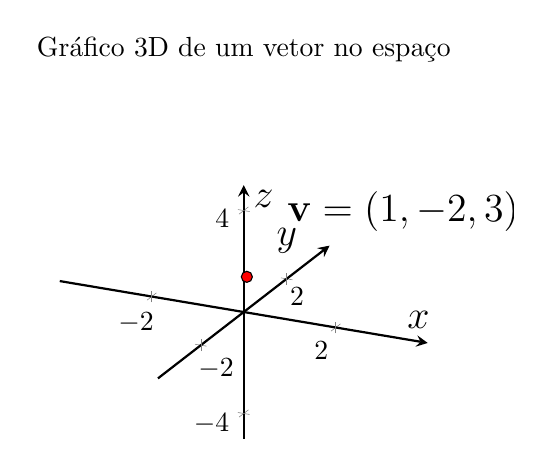
\begin{tikzpicture}
    \begin{axis}[
        axis lines = center,
        axis line style={thick},
        xlabel = {\Large $x$},
        ylabel = {\Large $y$},
        zlabel = {\Large $z$},
        xtick={-2,0,2},
        ytick={-2,0,2},
        ztick={-4,0,4},
        xmax = 4, xmin = -4,
        ymax = 4, ymin = -4,
        zmax = 5, zmin = -5,
        title={\normalsize Gráfico 3D de um vetor no espaço},
        grid=none
    ]
        % Desenhar ponto (1, -2, 3)
        \addplot3[
            only marks,
            mark=*,
            mark options={scale=1, fill=red},
        ] coordinates {(1, -2, 3)};
        % Mover o valor do rótulo para frente
        \node at (axis cs:1.9, -2.5, 5) [anchor=south west] {\Large $\mathbf{v} = (1, -2, 3)$};

        % Desenhar linhas tracejadas até os eixos
      %  \addplot3[dashed, thick] coordinates {(0, -2, 3) (1, -2, 3)};
      %  \addplot3[dashed, thick] coordinates {(1, 0, 3) (1, -2, 3)};
      %  \addplot3[dashed, thick] coordinates {(1, -2, 0) (1, -2, 3)};
    \end{axis}
\end{tikzpicture}


\subsection{Distancias entre pontos}

Exemplo:
$E \in R$, descreva os pontos dados pelas equações:
\begin{itemize}
     

\item[a.] $x=5$
\item[b.] $y =3$
\item[c.] $x^2 + y^2 = 1$
    $d((x,y)(0,0)) \rightarrow \sqrt{(x-0)^2 + (y-0)^2} = 1$ \\
    $\leftrightarrow \sqrt{x^2 + y^2} = 1 \leftrightarrow x^2 + y^2 = 1$ 

\end{itemize}

Exemplo: Que superficie em $R^3$ é representada pela seguinte equação?
\begin{itemize}
    \item[a.] $z=3$  \\ A equação $z=3$ representa o conjunto $\{(x,y,z) / z=3 \}$
    \item[b.] $y = 5$ \\ A equação $y=5$ representa um conjunto de todos os pontos do espaço que tem 2º coordenadas igual a 5.  
\end{itemize}

\subsubsection{Formula de Distancias}
\begin{figure}[!h]
    \centering
    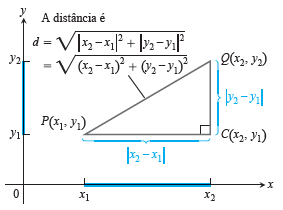
\includegraphics{sources/img/graficodistancia.png}
    \caption{Descrição da imagem}
    \label{fig:exemplo}
\end{figure}


\subsection{Esfera:}
\textbf{Definição}
Uma esfera de centro (a,b,c) e raio r é o conjunto de todos os pontos no espaço que estão a uma distancia e do ponto (a,b,c) e é descita por:
\begin{center}
\begin{align}
    \sqrt{(x-a)^2 + (y-b)^2 + (z-c)^2} = r^2 \leftrightarrow (x-a)^2 + (y-b)^2 + (z-c)^2 = r^2 
\end{align}
\end{center}

Exemplo: Mostre que $x^2 + y^2 + z^2 + 4x - 6y +2z + 6 = 0$ é a equação de uma esfera.
Identifique seu centro e raio. 
Solução: 
Podemos reescrever a e f fornecendo o seguinte modo.
$x^2 + 4x + y^2 -6y + z^2 +2z + 6 = 0 \leftrightarrow (x+2)^2  -4 + (y-3)^2 - 9 + (z+1)^2 -1 + 6 = 0$ \\
$(x+2)^2 + (y-3)^2 + (z+1)^2 = 8 \leftrightarrow (x-(-2))^2 + (y-3)^2 + (z-(-1))^2 = 8$ \\
Assim, a e f dado descreve os pontos da esfera de contro (-2,3,-1) e o raio $r=\sqrt{8}$

Exercicio: Determine a região em $\mathbb{R}$ decrita pelas inequações:
$1 \leq x^2 + y^2 + z^2 \leq 4$ e $ z \geq 0$

Exemplo: $E \in \mathbb{R}$ qual é a superficie decrita pela equação $x^2 + y^2 =1$. 
